\section{Diagramme de transition d'état}
	Une unité naît, meurt, et entre temps, fait la bagarre. Afin de comprendre son cycle de vie qui peut parfois être complexe, la Figure \ref{fig:transition_unit} illustre avec brio les transitions entre les différents états de l'unité.

	\begin{figure}[h!]
		\centering
		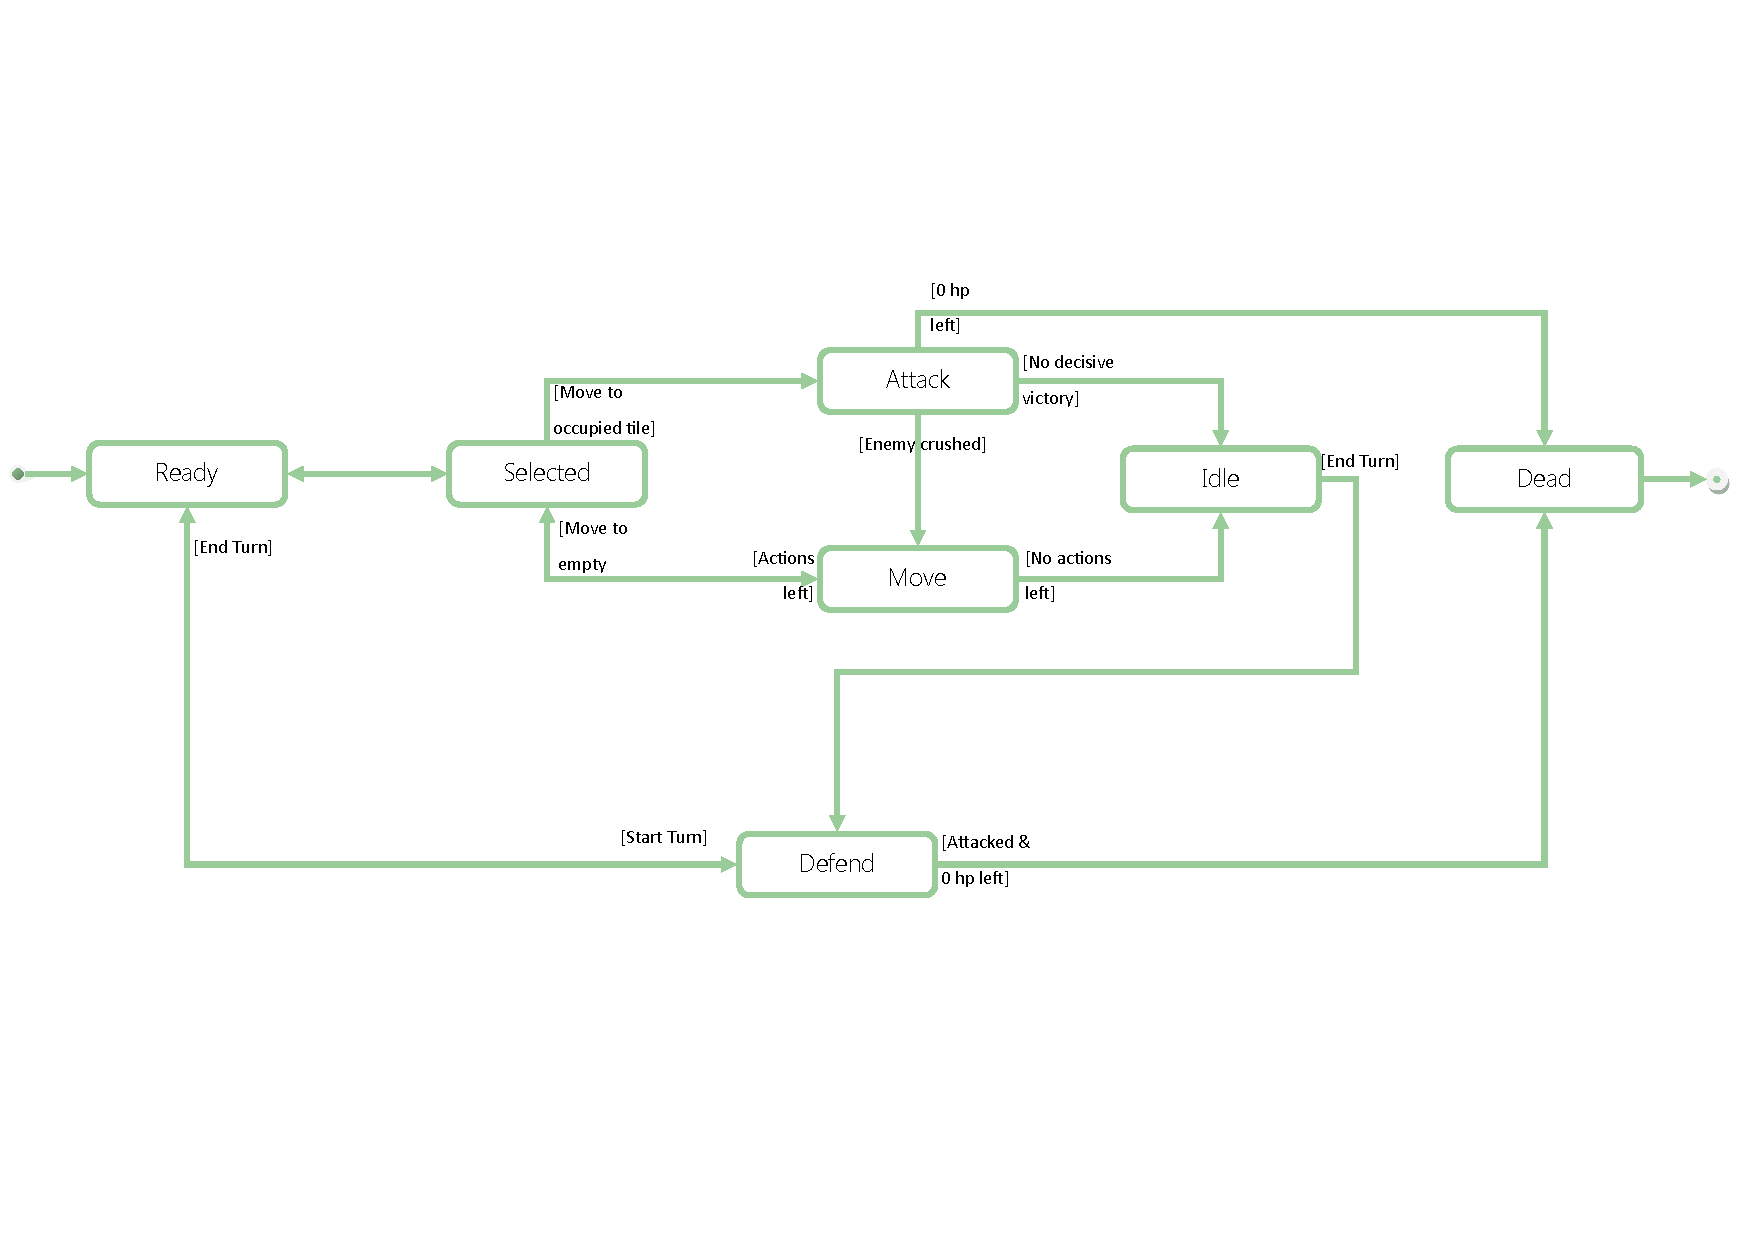
\includegraphics[width=1\textwidth]{figure/transition_unit.pdf}
		\caption{La médecine n'ayant pas été inventée, les unités ont aucun moyen de regagner leurs points de vie.}
		\label{fig:transition_unit}
	\end{figure}